\documentclass[12pt]{article}
\usepackage{amsmath, amsthm, amsfonts, amssymb}
\usepackage{graphicx} % for images
\usepackage{hyperref}

% Define theorem and lemma environments
\newtheorem{theorem}{Theorem}
\newtheorem{lemma}{Lemma}
\newtheorem{definition}{Definition}

\setlength{\parindent}{0pt}

\begin{document}

\title{Bayesian-Optimal Multi-Classification with Noisy Input Necessitates
General Input Space Representation}

\author{Aman Bhargava}

\date{\today}
\maketitle

\section{Introduction}
\textit{Notation: lower case variables denote scalars (e.g., $x$), upper case variables denote random variables (e.g., $X$), and boldfaced variables denote vector quantities (e.g., $\mathbf x, \mathbf X$).} \\

Here I analyze the latent representations in optimal Bayesian filter models
trained to perform multi-class classification on some ground truth input vector 
$\mathbf x^* = [x_1^*, x_2^*]^\top$ 
based on noisy discrete-time measurement signals
$\mathbf X(t) = [X_1(t), X_2(t)]^\top$ defined as  
\begin{align}
	\label{eqn:def_noisy_input}
	X_1(t) &= x_1^* + \eta \mathcal N(0, 1) \\
	X_2(t) &= x_2^* + \eta \mathcal N(0, 1) 
\end{align}
We scope our analysis to $N$ linear classification boundaries.
The multi-classification task may be defined in terms of $N$ classification
boundary angles $\alpha_1, \dots, \alpha_N $ which we collectively denote as $\Theta$: 
\begin{equation}
	\label{eqn:boundaries}
	\Theta = \{\alpha_i : \alpha_i \in [-\pi, \pi], i = 1, \dots, N\}
\end{equation}
as in Figure~\ref{fig:2a}. 
\begin{figure}[h! tbp]
	\centering 
	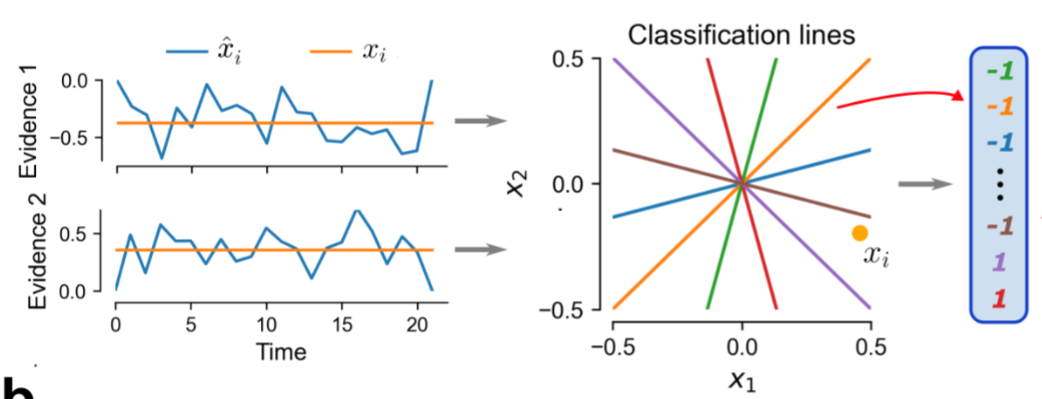
\includegraphics[width=0.9\textwidth]{media/multitask_fig2a.png}
	\caption[Multitasking RNN learns abstract representations]{\textbf{Multitasking RNN learns abstract representations. } Data generating process. The task is to simultaneously report whether the true joint evidence $(x_1,x_2)$ (yellow dot) lies above ($+1$) or below ($-1$) a number of classification lines (here 6).}
	\label{fig:2a}
\end{figure}
% The classification boundary for $\alpha_i$ is the line $x_2 = x_1 \tan \alpha_i$. 
Models are tasked with predicting the binary classification label for corresponding to each boundary in $\Theta$. 
We denote the $N$ labels $\mathbf y^* = [y_1^* \dots y_N^*]^\top$ 
corresponding to some $\mathbf x^*$ based on the resulting noisy measurement
signals $\mathbf X(t)$ where 
\begin{equation}
	\label{eqn:def_multiclass_output}
	y_i^* = \begin{cases}
		+1 & \text{ if $x_2^* > x_1^* \tan \alpha_i$} \\
		-1 & \text{ otherwise }
	\end{cases}
\end{equation}

\paragraph{Contribution: } In this document, I demonstrate that a
Bayesian-optimal multi-classifier with noisy random input $\mathbf X(t)$ and
classification estimate output $\hat {\mathbf y}(t) \in [-1, 1]^N$ must form
latent representations $\mathbf z(t)$ that retain the 2-dimensional structural
information of the input data space $[x_1^*, x_2^*] \in \mathbb R^2$ in the
limit as $N\to \infty$ for densely packed $\alpha_i \in \Theta$. 
Intriguingly, without noise, we are unable to guarantee that optimal latent
representations $\mathbf z(t)$ will retain sufficient information to estimate
$\mathbf x^*$. 
While the proof is stated for 2-dimensional input, the argument holds for
any input dimensionality. 


\subsection{Bayesian Filtering Framework}

Bayesian filters are a class of statistical models and algorithm that update a
latent state based on noisy and uncertain observation signals. 
Rooted in principles of Bayesian inference, these filters combine aggregated 
``knowledge'', represented by a latent state $\mathbf Z(t)$, with incoming
observations $\mathbf X(t)$ to continually update the latent state to
facilitate some prediction of some output $\mathbf Y(t) = f(\mathbf Z(t))$. 


\begin{definition}[Bayesian Filter Operation]
	\label{def:bayesian_filter}
	A discrete-time Bayesian filter updates latent variable $\mathbf z(t)$
	based on incoming data $\mathbf x(t)$ by applying Bayes' theorem: 
	\begin{align}
		\label{eqn:bayes_filter}
		P \big(\mathbf z(t) | \mathbf  x(t), \mathbf z(t-1)\big) &= \frac{
			P\big(\mathbf x(t) | \mathbf z(t), \mathbf z(t-1)\big) 
			P\big(\mathbf z(t) | \mathbf z(t-1)\big)
		}{
			P\big(\mathbf x(t) | \mathbf z(t-1)\big)
		} \\
		&\propto P\big(\mathbf x(t) | \mathbf z(t) \big) 
			P\big(\mathbf z(t) | \mathbf z(t-1)\big)
	\end{align}
	Bayesian filters are commonly equipped with a ``decoder'' or ``readout
	map'' $f$ which maps latent $\mathbf Z(t)$ to readout estimation
	$\hat{\mathbf Y}(t) = f(\mathbf Z(t))$.
\end{definition}

There is a deep structural similarity between RNNs and Bayesian filters, as
both models update some latent state $\mathbf z(t)$ based on incoming datum
$\mathbf x(t)$. 
Moreover, RNNs and Bayesian filters are both frequently used to predict some
value $\mathbf y(t) = f(\mathbf z(t))$ (citation: Goodfellow for RNN, Bayesian
inference textbook for filters).
We leverage the structure in the Bayesian filter formulation to prove our main
result in Section~\ref{sec:main}. 


\subsection{Canonical Bayesian Filtering Example}
A canonical example of Bayesian filtering is estimating the position of a robot based on noisy sensory readings (Figure~\ref{fig:robot_filter_ex}). 
Continuing with the same notation as above, assume the ground truth position of the robot is $\mathbf x^* \in \mathbb R^2$. 
We obtain noisy sensor readings $\mathbf X(t) = \mathbf x^* + \eta \mathcal N(\mathbf 0, \mathbb I)$, where $\eta$ is the amount of zero-mean, identity covariance noise. 
The latent variable $\mathbf Z(t)$ represents our estimate of $\mathbf x^*$ at time $t$. 
Using Equation~\ref{eqn:bayes_filter}, we obtain the updated estimated position based on incoming readings $\mathbf X(t)$. \\

\begin{figure}[h! tbp]
	\centering 
	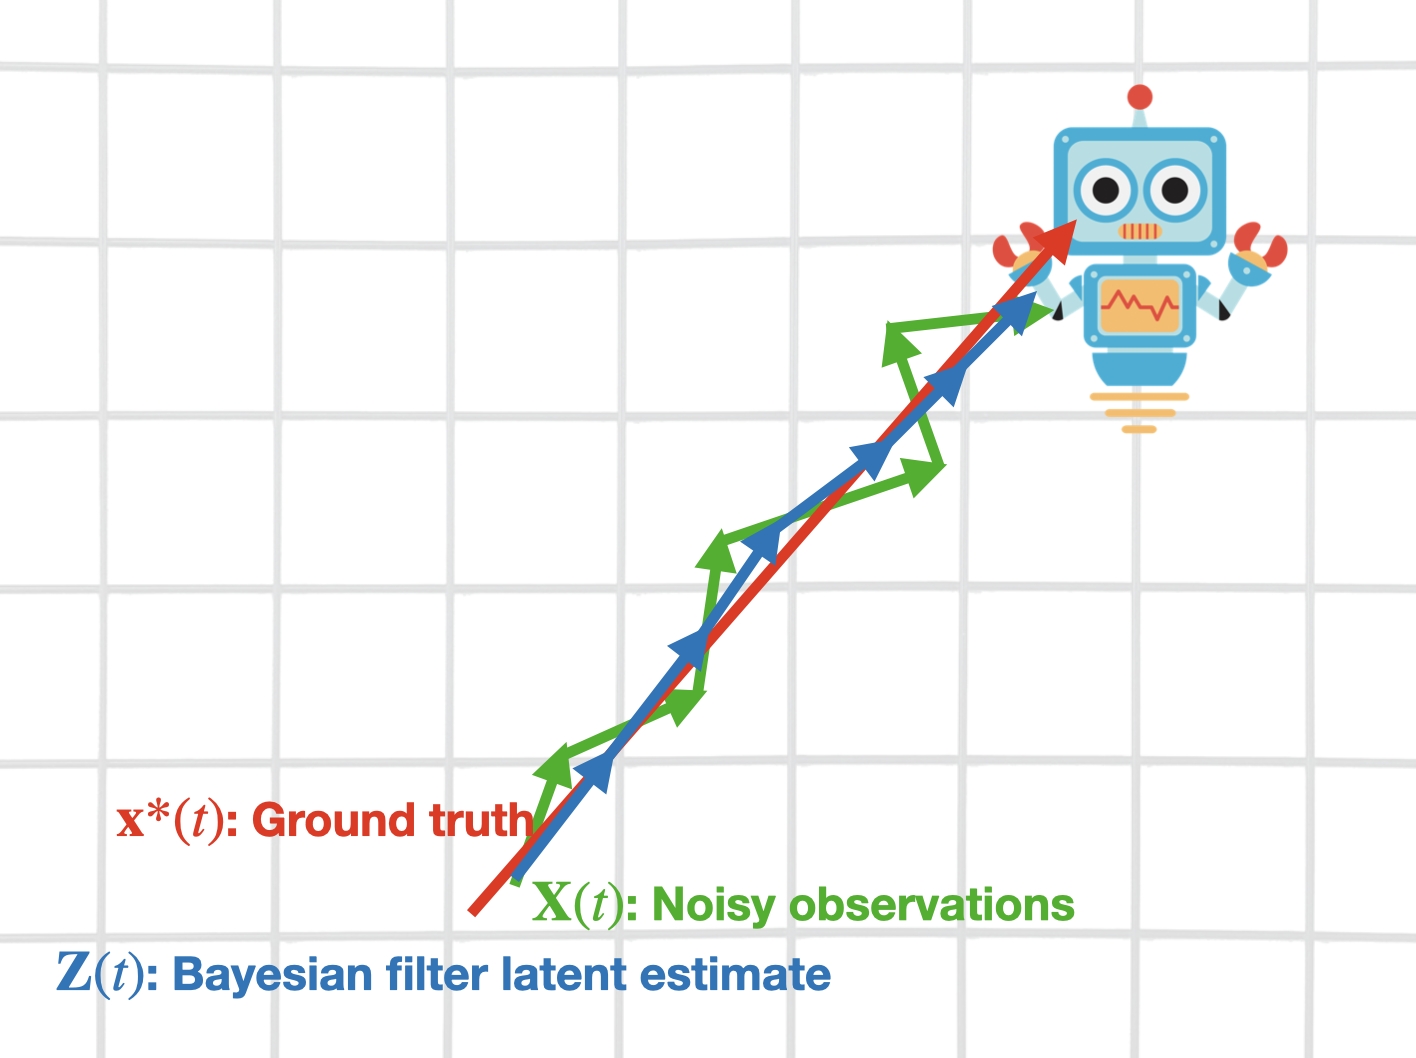
\includegraphics[width=0.5\textwidth]{media/robot_filter.png}
	\caption[Canonical filtering task]{This figure shows the estimation of ground truth trajectory $\mathbf x^*(t)$ based on noisy readings $\mathbf X(t)$. $Z(t)$ is shown in blue, representing the filtered estimate of $x^*(t)$ in red based on $\mathbf X(t)$ in green.}
	\label{fig:robot_filter_ex}
\end{figure}

In practice, we would initialize the latent variable $\mathbf Z(0) = \mathbf 0$ or some other neutral position. 
The prior distribution $P(\mathbf Z(t) | \mathbf Z(t-1))$ represents our belief about the robot's current position before seeing any new sensor data. 
We assume this is Gaussian-distributed around $\mathbf Z(t-1)$, though we can augment the sophistication of our prior model by including velocity and acceleration estimates (cf. Kalman filter). 
This added sophistication is how one may connect system state estimation (observer theory) to classic linear state space control theory. 
The likelihood function $P(\mathbf X(t) | \mathbf Z(t))$ represents the probability of observing a particular sensor reading given the current latent state $\mathbf Z(t)$. 
We assume this is Gaussian-distributed around $\mathbf Z(t)$. 
At each update step, the position estimate $\mathbf Z(t)$ is updated with the incoming data by combining the prior belief and the likelihood. \\ 

In neuroscience, this example parallels how the brain integrates information over time to refine its predictions over future states. 
This model highlights the probabilistic nature of perception and decision-making in the brain, illustrating how biological systems might deal with uncertainty and noise in sensory processing.
Analyzing Bayesian-optimal filters is therefore of great interest for understanding the properties of high-performance iterative information processing systems -- particularly those performing prediction tasks on uncertain/noisy input.


\section{Main Results}
\label{sec:main}

Consider an optimal Bayesian filter for the multi-class classification task
$\Theta$ on noisy discrete time measurement signals. 
Let $\epsilon$ be the maximum angular gap between classification boundaries in $\Theta=(\alpha_1 \dots \alpha_n)$ (Definition~\ref{def:epsilon}).

\begin{equation}
	\label{def:epsilon}
	\epsilon = \max_{i \in N} \min_{j > i} \| \alpha_i - \alpha_j \|
\end{equation}

\begin{theorem}
	\label{thm:main}
	An optimal Bayesian filter trained to perform multi-class classification on
	ground truth input $\mathbf x^*$ w.r.t. decision boundaries 
	$\Theta = \{\alpha_1, \dots, \alpha_N\}$ based on noisy measurement signals
	$\mathbf X(t)$ must have latent state $\mathbf Z(t)$ that retains a
	representation of the 2-dimensional input vector $\mathbf x^*$ in the limit 
	as $\epsilon \to 0$. 
\end{theorem}

\begin{proof}
	\begin{lemma}[Equivalence to Angle Estimation]
		\label{lemma:angle_equiv}
		In the limit as $\epsilon \to 0$ for decision boundaries $\Theta =
		(\alpha_1, \dots, \alpha_N)$, the multi-classification task of
		estimating $\mathbf y^*$ (Equation~\ref{eqn:boundaries}) for a given
		$\mathbf x^*$ given noisy observations $\mathbf X(t)$ is equivalent to
		estimating the angle $\theta = \angle \mathbf x^*$. 
	\end{lemma}


	\begin{lemma}[Angle Estimation Requires Magnitude Estimation]
		\label{lemma:angle_to_magnitude}
		An optimal Bayesian filter predicting the angle of some ground truth
		input $\angle \mathbf x^*$ based on noisy observations $\mathbf X(t)$
		must implicitly estimate the magnitude of $\mathbf x^*$ during state
		updates on latent variable $\mathbf Z(t)$. 
	\end{lemma}
	\begin{proof}
		We denote the conditional entropy of angle estimate $\hat \theta =
		f(\mathbf Z(t))$ as $H(\hat \theta | \mathbf Z(t))=  H(\hat \theta |
		\mathbf X(1), \dots, \mathbf X(t))$.
		Since $\mathbf X(t)$ is subject to equivariant Gaussian noise with
		variance $\eta$, the condition entropy is inversely proportional to the
		distance between point $x^*$ and classification boundaries $\Theta =
		(\alpha_1, \dots, \alpha_N)$.  
		For fixed angle $\theta = \angle \mathbf x^*$, the distance between
		$\mathbf x^*$ and each classification boundary scales monotonically
		with $\|\mathbf x^*\|$. 
		Therefore, the angle $\angle \mathbf x^*$ and the entropy of the angle
		estimate $H(\hat \theta | \mathbf X(t) \dots \mathbf X(t)) = H(\hat
		\theta | \mathbf Z(t))$ is sufficient to determine $\|\mathbf x^*\|$. 
		Since $\hat \theta$ and $H(\hat \theta | Z(t))$ are both functions of
		$\mathbf Z(t)$ and $\lim_{t\to\infty}\hat \theta = \theta$ we have demonstrated that
		$\mathbf Z(t)$ implicitly estimates the magnitude of $\mathbf x^*$.
	\end{proof}

	Therefore, multi-class classification in the limit as the decision boundary
	spacing $\epsilon \to 0$ is equivalent to estimating the angle of the
	ground truth $\mathbf x^*$ based on noisy $\mathbf X(t)$
	(Lemma~\ref{lemma:angle_equiv}).
	Optimal Bayesian filtering to estimate the angle $\theta = \angle \mathbf
	x^*$ also implies estimating the magnitude of the ground truth data
	$\|\mathbf x^*\|$. \\


	Thus we have demonstrated that both the angle information and the magnitude
	information of $\mathbf x^*$ must be implicitly estimated by an optimal
	Bayesian filter in multi-class classification problem $\Theta$ with
	non-zero equivariant noise $\eta$ in the measurements $\mathbf X(t)$. 
\end{proof}



\section{Discussion}

\subsection{Implications of Non-Equivariant Gaussian Noise}
In our analysis, we assumed equivariant Gaussian noise with variance $\eta$ in
$\mathbf X(t)$. 
The case of $\eta = [\eta_1, \eta_2]^\top$ with $\eta_1\neq\eta_2$ can be made
equiavlent to the equivariant case via a coordinate transformation $x_2 = x_2
\eta_1 / \eta_2$. 
This may change the maximum inter-classification boundary distance $\epsilon$, 
but the final result remains the same as $\epsilon \to 0$. 


\subsection{Generalizing to Higher Dimensions}
To generalize these results to higher dimensions, the Lemmas~\ref{lemma:angle_equiv} and \ref{lemma:angle_to_magnitude} must be expanded. 
Lemma~\ref{lemma:angle_equiv} focuses on the equivalence of the multi-classification problem to angle estimation. 
This condition can be expressed for a high dimensional space in terms of hyperplane decision boundaries passing through the origin. 
The angle estimation problem becomes a multi-angle estimation problem (e.g., latitude and longitude for $\mathbb R^3$). 
The condition on maximal angular spacing $\epsilon \to 0$ can be generalized as an upper bound on surface area of the slices of a sphere defined by the hyperplanes' intersection with a sphere centered on the origin. 

\subsection{Implications for Learned Representations in the Brain}
This theoretical analysis implies a connection between multi-task learning and topological information preservation in optimal Bayesian filtering models. 
Understanding how representations of an underlying statistical process emerge in information processing systems is central to understanding cognition. 
Our results suggest that a multi-tasking system must learn a representation of incoming noisy data that preserves the central aspects of the underlying topology of the statistical process.
This harkens to work on the automated construction of cognitive maps via predictive coding (\href{https://www.biorxiv.org/content/10.1101/2023.09.18.558369v1}{Gornet and Thomson, 2023}). 
In their paper, ``Automated construction of cognitive maps with predictive coding'', Gornet and Thomson demonstrate predictive coding (i.e., predicting subsequent sensory input) is sufficient for an agent to form an internal \textit{map} of its environment. 
Our work suggests a relaxed condition -- that, under certain conditions, multi-task classification may also yield topology-preserving representations of the environment. 
Further work is warranted to determine the precise relationship between these concepts. 

\subsection{Relationships between $H(\mathbf X(t))$ and $H(\mathbf Z(t))$}
The goal of optimal Bayesian filtering is to maximize \textit{information gain} $IG$. 
\begin{equation}
	\label{eqn:info_gain}
	IG = 
		\underbrace{H(P(\mathbf Z(t) | \mathbf Z(t-1)))}_{\text{Prior}}
		-
		\underbrace{H(P(\mathbf Z(t) | \mathbf X(t), \mathbf Z(t-1)))}_{\text{Posterior}}
\end{equation}

Maximizing information gain can be understood as minimizing the entropy (uncertainty) of the posterior distribution.

As the posterior is proportional to the likelihood $P(\mathbf X(t) | \mathbf Z(t))$, it is tempting to relate the entropy of the likelihood -- i.e., the ability to predict incoming data -- and the posterior. 
Unfortunately, due to the interplay between the prior and the likelihood, the relationship between the entropy of the likelihood and the entropy of the posterior is not straight forward. 



\section{Information Theoretic Analysis of Main Result}

Our main result revolves around demonstrating that Bayes-optimal multi-task classification implies latent variable $\mathbf Z(t)$ from which the input coordinate $\mathbf X(t)$ could be recovered. 
Let us zoom out on the full graphical model representing Bayesian filter: 

\begin{figure}[h! tbp]
	\centering 
	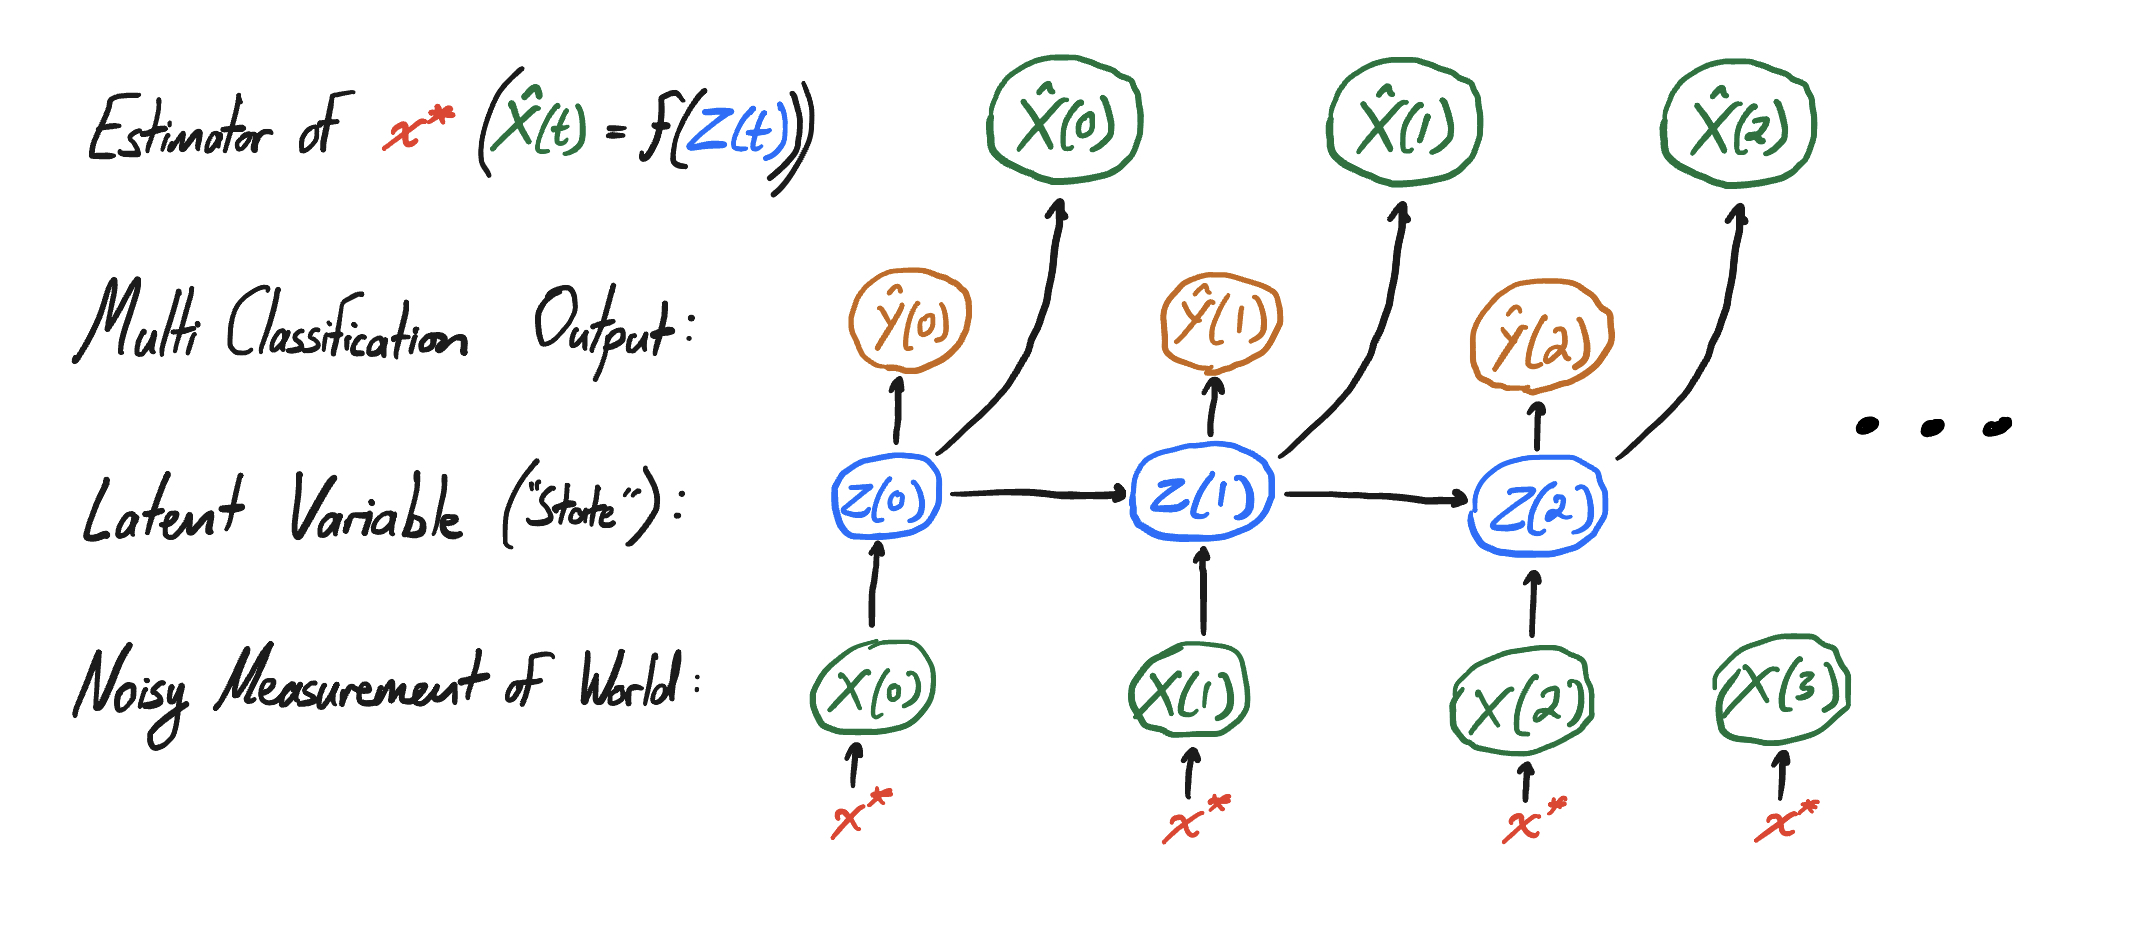
\includegraphics[width=0.99\textwidth]{media/bayesian_filter_graphical_model.jpg}
	\caption[Bayesian Filter Graphical Model]{
		\textbf{Multi-task Bayesian filter Graphical Model:} Graphical model representation of the multi-task filtering task. 
	}
	\label{fig:2a}
\end{figure}

Our result can be expressed in terms of the mutual information between random variables $\mathbf Z(t), \mathbf X(t) = \mathcal N (\mathbf x^*, \eta \mathbb I)$ and a hypothetical $\hat{\mathbf X}(t) = f(\mathbf Z(t))$ that is a deterministic function of latent $\mathbf Z(t)$. 


\section{Trilateration Trick for Recovering $\hat{\mathbf X}$ from $\mathbf Z(t)$}
In generalizing our main result, I found it helpful to introduce the idea of \textit{triangulation} of the position of the ground truth $\mathbf x^*$. 
Triangulation is when you constrain a position based on known distances to known points. 

\begin{theorem}
	\label{thm:trilateration}
	The sample entropies of each classification output $P(\hat{\mathbf Y})$ in a Bayesian-optimal is sufficient to trilaterate $\mathbf x^*$ w.r.t. $D+1$ decision boundaries where $D$ is the dimension of the underlying space $\mathbf x^*$ assuming sensor readings $\mathbf X(t)$ is subject to equivariant Gaussian noise.
\end{theorem}



\end{document}
